%! Author = ewan
%! Date = 10/6/25

% Preamble
\documentclass[11pt]{article}

% Packages
\usepackage{amsmath}
\usepackage{xcolor}
\usepackage{hyperref}
\usepackage{pdfpages}
\usepackage{graphicx}
\usepackage[toc,page]{appendix}
\usepackage{caption}


% Document
% Document
\begin{document}

    \title{
            { \textbf{Security Protocols and Verification}} \\[1ex]
        {\small Defense of Cryptographic Protocol}
    }


    \author{
        Garance Frolla \\
        Ely Marthouret \\
        Ewan Decima\\ \\
        Team: \textbf{ASKO OM8464A2}
    }

    \date{September / November 2025}


    \maketitle
    \tableofcontents
    \newpage

    \section{Attack against PROTOxyde d'alCOl}

    \subsection{Notation}
    \begin{itemize}
        \item Let $\mathcal{K}_I$ denote the set of all facts known to the intruder $I$.
        \item Let $\bigl(K_I\bigr)_{I \in \mathcal{I}}$ the set of key use by $I$ during the \textit{bruteforce} step.
        \item Let $\mathcal{M}$ denote the set of all  messages sent during a communication between to agents.
        \item Let $M_{1,A} \in \mathcal{M}$ denote the first message sends by Alice, i.e., $M_{1,A} = \{|\langle A,N_A \rangle|\}_{K_{AB}}$
        \item Let $s(\cdot, \cdot)$ denote the sender function, i.e., $s(m,x)$ means message $M$ is sent by agent $C$.
        \item Let $[\cdot]_{(\cdot)}$ denote the extract function of a tuple message, i.e., for
                $ M = \langle m_1, m2, ..., m_n \rangle \in \mathcal{M}$, $[M]_i = m_i \quad \forall i \in [|1,n|]$.
        \item Let $\langle X',Y',Z', \Sigma' \rangle$ denote four random value.
    \end{itemize}
    

    \subsection{The attack}
    \begin{itemize}
        \item First this our understanding of your attack : the intruder $I$ steal the first alice's message :
        $M_{1,A}$. At this step $ K(N_A) \notin \mathcal{K}_I  $ and $K\bigl(K_{AB}\bigr) \notin \mathcal{K}_I$.


        \item After that, $I$ impersonates S by crafting the ticket $\{|\langle A,\tau,\lambda, K_{AB}\rangle|\}_{K_{BS}}$,
                replacing $K_{BS}$ with keys $K_I$ to form $T_I := \{|\langle X',Y',Z', \Sigma' \rangle|\}_{K_{I}}$
            and sending $M_{1,A}$ and $T_I$ to $B$.
        
        \item $B$ gets $M_{1,A}$. At this point $K\bigl( S(M_{1,A},A) \bigr) \notin \mathcal{K}_B$.
                But it's normal according to the ASKO OM8464A2 protocol. Then $B$ gets the crafted ticket $T_I$. $B$
                will decipher it with $K_{BS}$ and send back to $[dec(T_I, K_{BS})]_1$
                \begin{center}
                    $\Bigl\{\Bigl|dec\bigl(\{|N_A + 1|\}_K_{AB},[dec(T_I, K_{BS})]_4\bigr) \Bigr|\Bigr\}_{[dec(T_I, K_{BS})]_4}$
                \end{center}
        For better understanding, let us denote $[dec(T_I, K_{BS})]_1$, $[dec(T_I, K_{BS})]_2$, $[dec(T_I, K_{BS})]_3$, $[dec(T_I, K_{BS})]_4$
        as $X,Y,Z,\Sigma$ respectively.


        \item The attack lies on the fact that identities are short bitstring,  $B$ will always decipher the ticket
                $T_I$ with his symmetric key $K_{BS}$, and hoping that:
                \begin{center}
                    $\exists \: J \in \mathcal{I} \: | J \neq BS \wedge \: dec(T_J, K_{BS}) = \langle A,Y,Z, \Sigma \rangle$.
                \end{center}
                With such a key $K_J$, $B$ will think that $\Sigma$ is $K_{AB}$. At this point $K\bigl(\Sigma \bigr) \notin \mathcal{K}_I$
                and $K\bigr( K_J \bigl) \notin \mathcal{K}_I$.

    \end{itemize}

    \section{Refutation}
        \subsection{Symmetric encryption specification}



            The assumption that if $B$ uses a different key $K_{BS} \neq K_I$ that the one used for encryption of $T_I$ by the
            intruder the decrypted output will be garbage (random-looking bytes) is questionable and depend a lot of
            the code implementation of the protocol. In fact, if the implementation uses an authenticated mode,
            like AES-GCM or ChaCha20-Poly135, decryption will fail completely. But if the implementation uses AES-CBC
            it won't throw an error and $B$ will get nonsense plaintext.

            \vspace{0.5cm}

            Moreover if $I$ uses the wrong cipher configuration such ad AES-ECB instead of AES-CB or AES-GCM, $B$ will
            end up with completely unreadable results, and if the padding is incorrect (for example, PKCS7 was expected
            but not applied), $B$ will likely encounter padding errors or corrupted trailing bytes.

            \vspace{0.5cm}

            Finally, if $I$ uses the wrong Initial Vector (IV) or nonce, the first block (or few blocks) of
            decrypted data will be corrupted. The rest might still decrypt correctly depending on the mode (e.g., CBC
            mode propagates errors, but CTR mode only corrupts corresponding parts)



            \vspace{0.5cm}

            Since the protocol design project did not require us to specify the actual implementation of the protocol
            but only its theoretical aspect, the choice of the encryption scheme cannot be considered a point of attack;
            we can assume the encryption scheme to be flawless. For example in the Needham-Schroeder template, there is
            no mention of the encryption scheme.


    \subsection{Litterature}

    In cryptographic literature, and particularly in theoretical descriptions of protocols (for key exchange,
    authentication, etc.), there are no specifications regarding the choice of implementation or hardware aspects. For
    example, in \textit{Applied Cryptography, Second Edition} by Bruce Schneier (translated by Laurent Viennot), in the
    section 'Authentication and Key Exchange,' the theoretical description of the Needham–Schroeder protocol does not
    mention the choice of the symmetric encryption algorithm, nor the size used to encode the participants’ identities.
    (\textit{See ~\ref{fig:NS_BS} in Appendices~\ref{ann:NS_BS}})



    \subsection{Timestamp}
    

    
    \subsection{Bruteforce issues}
        First of all $K_{BS} \notin \mathcal{K}_I$. $I$ can try to bruteforce $K_{BS}$ but we don't think that $I$ will outlive \textit{Dracula}.
    
    %- litteratre
    %- validity of the timestamp
    %- aes failure
    %- B send not tp A at every time and I dont know to who B will send the answer

    
    \section{Conclusion}
    We refuse the attack.


    \newpage
    \begin{appendices}

        \section{Theoretical Needham-Schroeder}\label{ann:NS_BS}


        \begin{figure}[h!]
            \centering
            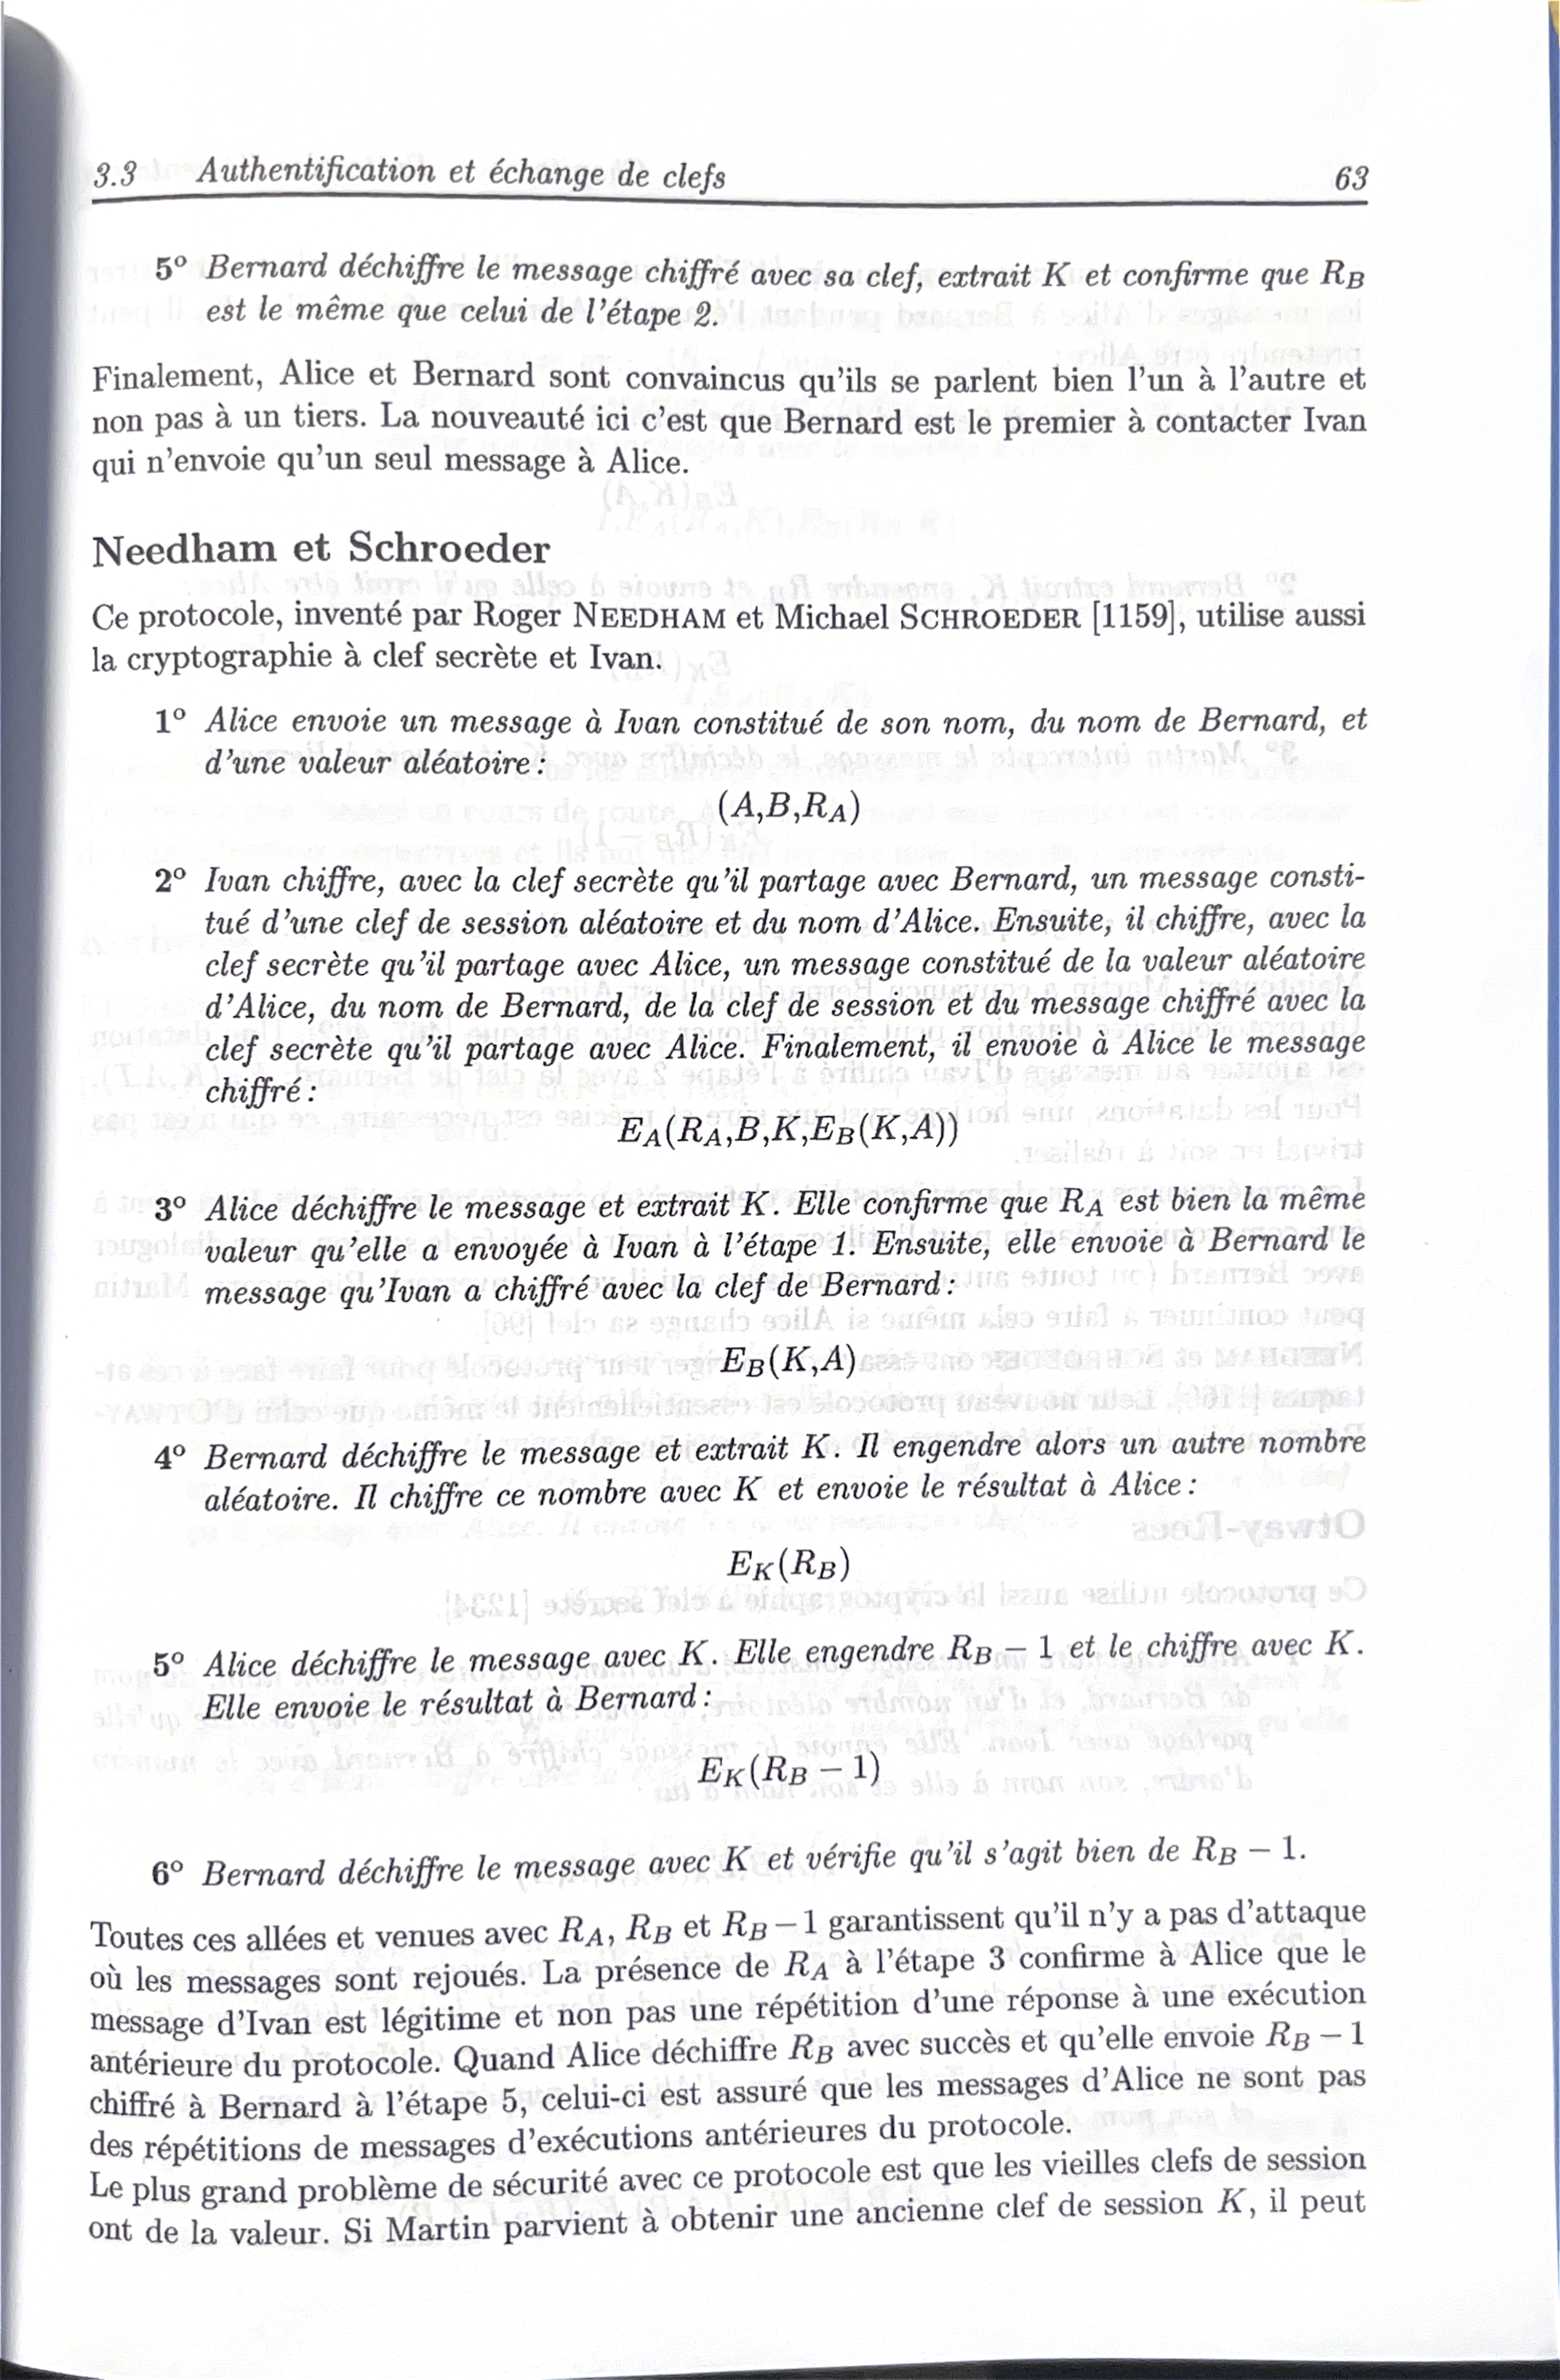
\includegraphics[width=0.8\textwidth]{NS-schneir}
            \caption{NS in \textit{Applied Cryptography} by Bruce Schneier}
            \label{fig:NS_BS}
        \end{figure}

    \end{appendices}


\end{document}